\section{Auswertung}
\label{sec:Auswertung}

Im nun Folgenden werden die aufgenommenen Messdaten der verschiedenen Scans ausgewertet. 


\subsection{Detektorscan}
\label{sec:Detektorscan}

Zu Beginn wird anhand des Detektorscans die Halbwertsbreite und die maximale Intensität bestimmt.
Hierfür wird eine Gaußfunktion der Form
\begin{equation}
    I(\theta)= a \cdot \exp \left(-\frac{(\theta-\mu)^2}{b}\right)
\end{equation}
als Regression an die Messdaten verwendet,
die in \autoref{fig:Detektorscan} zu sehen ist.
\begin{figure}
    \centering
    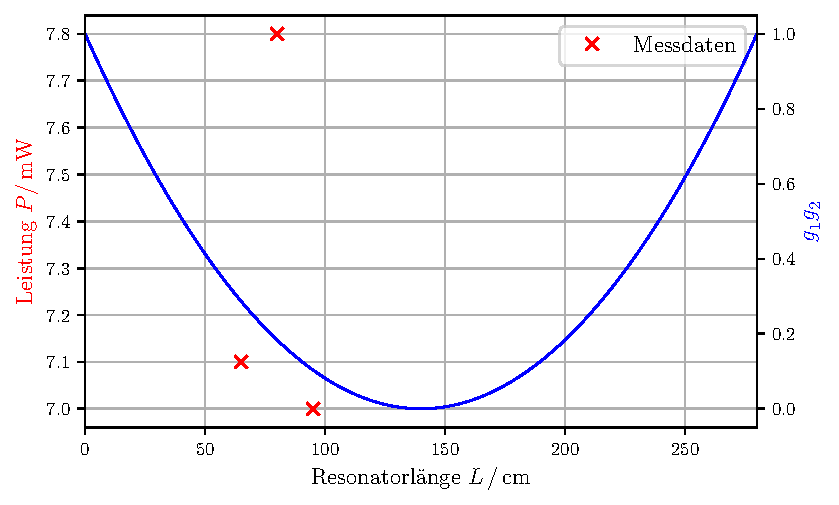
\includegraphics[width = 0.8\linewidth]{build/plot1.pdf}
    \caption{Messdaten des Detektorscans mit Regression und FWHM.}
    \label{fig:plot1}
\end{figure}

Die daraus resultierenden Parameter ergeben sich zu 
\begin{align*}
    a & = \qty{0.95784(9)}{} \, , \\
    b & = \qty{0.0028(6)}{} \, , \\
    \mu & = \qty{0.001(14)}{\degree} \, .
\end{align*}

Mittels der Phyton-Bibliothek \textit{SciPy} \cite{scipy} ergeben sich die Halbwertsbreite FWHM
und die maximale Intensität $I_\text{max}$ zu
\begin{align*}
    \text{FWHM} & = \qty{0.0879}{\degree} \quad \text{und} \\
    I_\text{max} & = \num{4.85e5} \, \# \, / \, \unit{\second} \, .
\end{align*}


\subsection{Z-Scan}

Mithilfe des ersten 